\documentclass[tikz,border=7pt]{standalone}
\usepackage[scaled=0.95]{helvet}
\renewcommand{\familydefault}{\sfdefault}
\usepackage[europeanresistors,americanvoltages]{circuitikz}
\definecolor{TEJNavy}{HTML}{1E2B55}
\definecolor{TEJBlue}{HTML}{1769AA}
\begin{document}
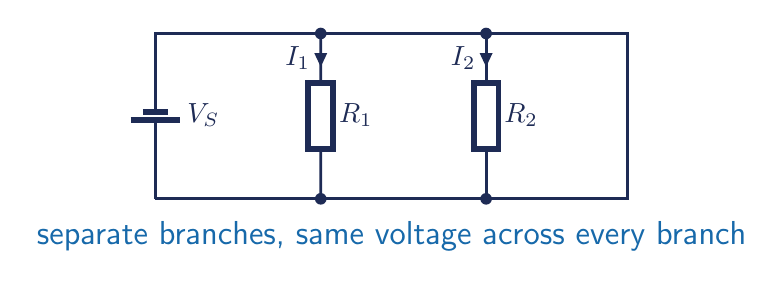
\begin{tikzpicture}[line width=1.05pt,draw=TEJNavy,text=TEJNavy]
  \ctikzset{bipoles/length=1.05cm}
  \draw
    (0,0) to[battery1,l_=$V_S$] (0,2.1)
    -- (6.0,2.1) -- (6.0,0) -- (0,0);
  \draw (2.1,2.1) to[R,l=$R_1$,i>_=$I_1$] (2.1,0);
  \draw (4.2,2.1) to[R,l=$R_2$,i>_=$I_2$] (4.2,0);
  \fill[TEJNavy] (2.1,2.1) circle (2.1pt) (2.1,0) circle (2.1pt)
    (4.2,2.1) circle (2.1pt) (4.2,0) circle (2.1pt);
  \node[font=\large,text=TEJBlue] at (3.0,-0.48)
    {separate branches, same voltage across every branch};
\end{tikzpicture}
\end{document}
